\chapter{Requirements Elicitation}
\label{ch:RequirementsElicitation}

As described in Chapter \ref{ch:RelatedWork}, recent research has identified several drawbacks to modern Web APIs. Studies have been conducted, showing that their evolution has a large impact on their consumers (\cite{brito_you_2020}, \cite{xavier_historical_2017}, \cite{espinha_web_2014}). As a consequence, client developers face an increased effort to keep their application code compatible, since current tools for the automatic migration of client code (\cite{henkel_catchup!_2005}, \cite{hutchison_automated_2006}) are not applicable in a Web API context \cite{li_how_2013}. In order to better understand Web API evolution, recent studies have introduced classifications of several recurring change patterns and evolution strategies that indicate the challenges providers and consumers are facing (\cite{li_how_2013}, \cite{lubke_interface_2019}). 

Addressing these challenges, we propose introducing a tool-supported workflow as shown in Figure \ref{fig:newWorkflow} to significantly reduce the impact of Web API evolution on consumers. Therefore, a majority of migratory tasks needs to be automated according to a machine-readable migration guide which needs to be prepared in advance by providers. All changes are encapsulated in a separate library to be abstracted from client code. This library is added to client applications as a dependency. In addition, our system facilitates the workflow of API providers to release new versions by ensuring that changes to the interface do not affect consumer applications, hence providing perceived stability. The system's main objective is to combine the convenience of local libraries with the flexiblity of modern Web APIs. It aims to be seamlessly integrated into commonly used tools and workflows like continuous integration, version control and dependency management. 

Given the current and proposed workflow, multiple functional and nonfunctional requirements can directly be derived. Web API consumers use the system to automatically migrate their application between two versions. Therefore, the system needs to import a machine-readable migration guide that is delivered by Web API providers. Our analysis identified all necessary system requirements which are listed in the following section in detail. Furthermore, use cases are identified for all actors and exemplary scenarios for possible future migration scenarios are presented. All requirements and constraints are listed in section \ref{sec:Requirements} while use cases and scenarios are shown in section \ref{sec:UseCases} and section \ref{sec:Scenarios}, respectively.
\newpage
\section{Requirements}
\label{sec:Requirements}

The system consists of two key components: a migration tool and a migration guide specification. This section provides an overview of the requirements and constraints for both of them. The system must meet all of them in order to be accepted. The requirements are split into functional and nonfunctional requirements. Bruegge et. al define functional requirements "[as] the interactions between the system and its environment independent of its implementation" \cite{bruegge_object-oriented_2010}. The authors thereby describe users and external systems as part of a system's environment. Furthermore, Bruegge et al. define nonfunctional requirements "as aspects of the system that are not directly related to the functional behavior of the system" \cite{bruegge_object-oriented_2010}. They further divide nonfunctional requirements into quality requirements and constraints. 

\subsection{Functional Requirements}
\label{subsec:FunctionalRequirements}
 
 In order to enable the implementation of the workflow shown in Figure \ref{fig:newWorkflow}, both, the functional requirements of the Web API consumers and providers must be taken into account. 

\begin{itemize}[itemindent=-4pt, leftmargin=34pt, align=left]
    \item [FR1\hphantom{1}] \customlabel{fr:MigGuide}{Developing a specification for a machine-readable migration guide (FR1)} \textbf{Development of a specification for a machine-readable migration guide:} The machine-readable migration guide needs to contain all necessary information regarding changes made to the Web API. Additionally, it must provide fields to specify important meta-data like versioning information. The format of the migration guide must allow the specification of simple and complex data structures. They are required to model hierarchies within the guide or hierarchical types provided by a Web API. Changes stated within the migration guide must be distinguishable from one another by their structure. Depending on its type, a change must include fields that contain information on how to adapt the client code to maintain compatibility with the Web API.
    \item [FR2\hphantom{1}] \customlabel{fr:Configuration}{Configuration} \textbf{Provide configuration option:} A user can configure the system by providing command-line parameters or a configuration file. If applicable, a default value is used in case of a missing configuration. For each API and project, an individual configuration can be applied.
    \item [FR3\hphantom{1}] \customlabel{fr:GenLib}{Generate a client library from service specification} \textbf{Generating a client library from service specification:} A user provides a Web API specification URI as input to generate a client library which can be used by the client application. The input can either be issued locally as a file or can be remotely retrieved from the web service.
    \item [FR4\hphantom{1}] \customlabel{fr:Facade}{Providing a facade to maintain API consistency (FR4)} \textbf{Provide a facade to maintain API consistency:} A user accesses the library's functionality via a generated facade to ensure a consistent view of the API. It mimics the original interface as it uses the same method signatures and exposes them to the client application.
     \item [FR5\hphantom{1}] \customlabel{fr:AdaptFacade}{Self-adapting facade for API evolution (FR5)}
     \textbf{Self-adapting facade for API evolution:} The system automatically resolves the current version of the web service and its corresponding migration guide. If the retrieved API version differs from the local API version, the system adapts the facade according to the migration guide. As a result, users automatically receive API-related changes in their application code.
     \item [FR6\hphantom{1}] \customlabel{fr:CIInteg}{Integrate system in CI/CD}
     \textbf{Integrate system in CI/CD:} The tool will be integrated into the CI pipeline of the client application to ensure the highest level of automation. Alternatively it can be used locally via its \textit{\ac{CLI}}.
     \item [FR7\hphantom{1}] \customlabel{fr:GitInteg}{Integrate output via Git}
     \textbf{Integrate output via Git:} The modified library will be published via git pull request into the client application's repository. By publishing it, the library's version number will be incremented according to semantic versioning principles.
     \item [FR8\hphantom{1}] \customlabel{fr:MigStrategy}{Specify migration strategy}
     \textbf{Specify migration strategy:} A user can specify the migration strategy for non-migratable changes such as deletion of functionality without replacement. The selected strategy can be either provided via command-line parameters or using the configuration file. 
          \item [FR9\hphantom{1}] \customlabel{fr:OutputLang}{Specify output language}
     \textbf{Specify output language:} A user can specify the programming language in which the target library is generated. The selected output language can be either provided via command-line parameters or using the configuration file. 
\end{itemize}

\subsection{Artifacts}
\label{subsec:Artifacts}

To illustrate the artifacts from FR1 and FR4, Figure \ref{fig:migGuide} shows our proposed structure for a machine-readable migration guide and Figure \ref{fig:outcome} demonstrates the architectural composition of the code generated by our system.

\begin{figure}[h]
	\centering{
		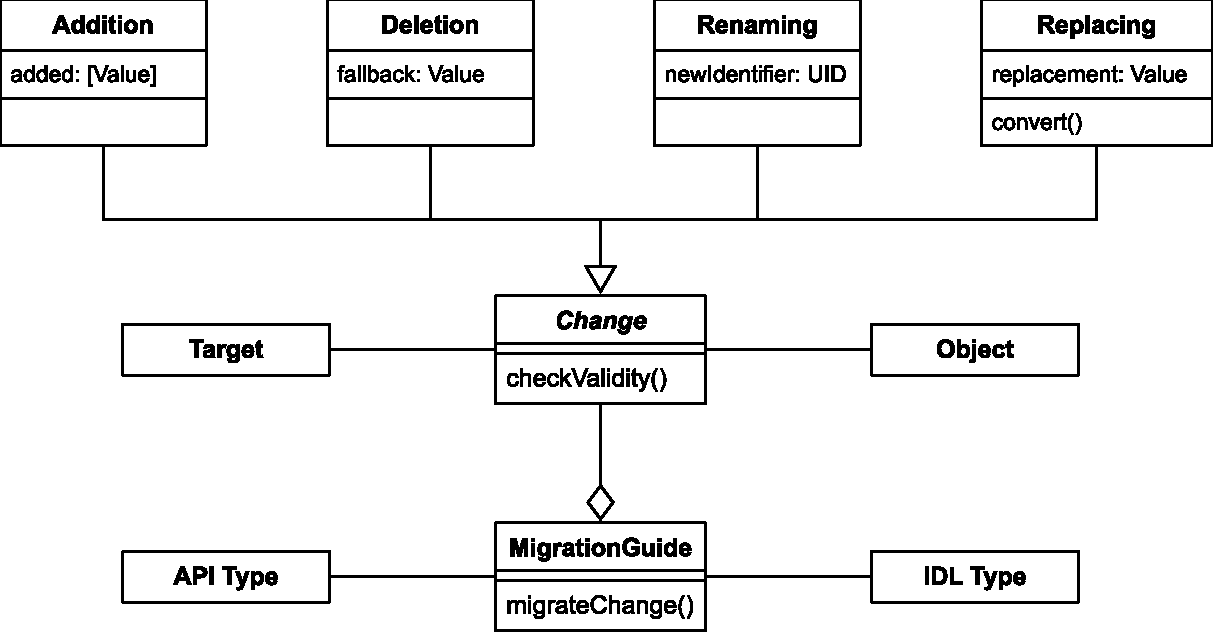
\includegraphics[width=135mm]{images/cd_migration_guide.pdf}
		\caption{Proposed structure of a machine-readable migration guide}
		\label{fig:migGuide}
	}
\end{figure}

A migration guide is responsible for migrating different types of changes that might occur due to Web API evolution. Each change must contain an identification of the object which is changed and the specific target of the change. For example, if a method parameter was changed, the method is the change object and the parameter is the change target.

\begin{figure}[!h]
	\centering{
		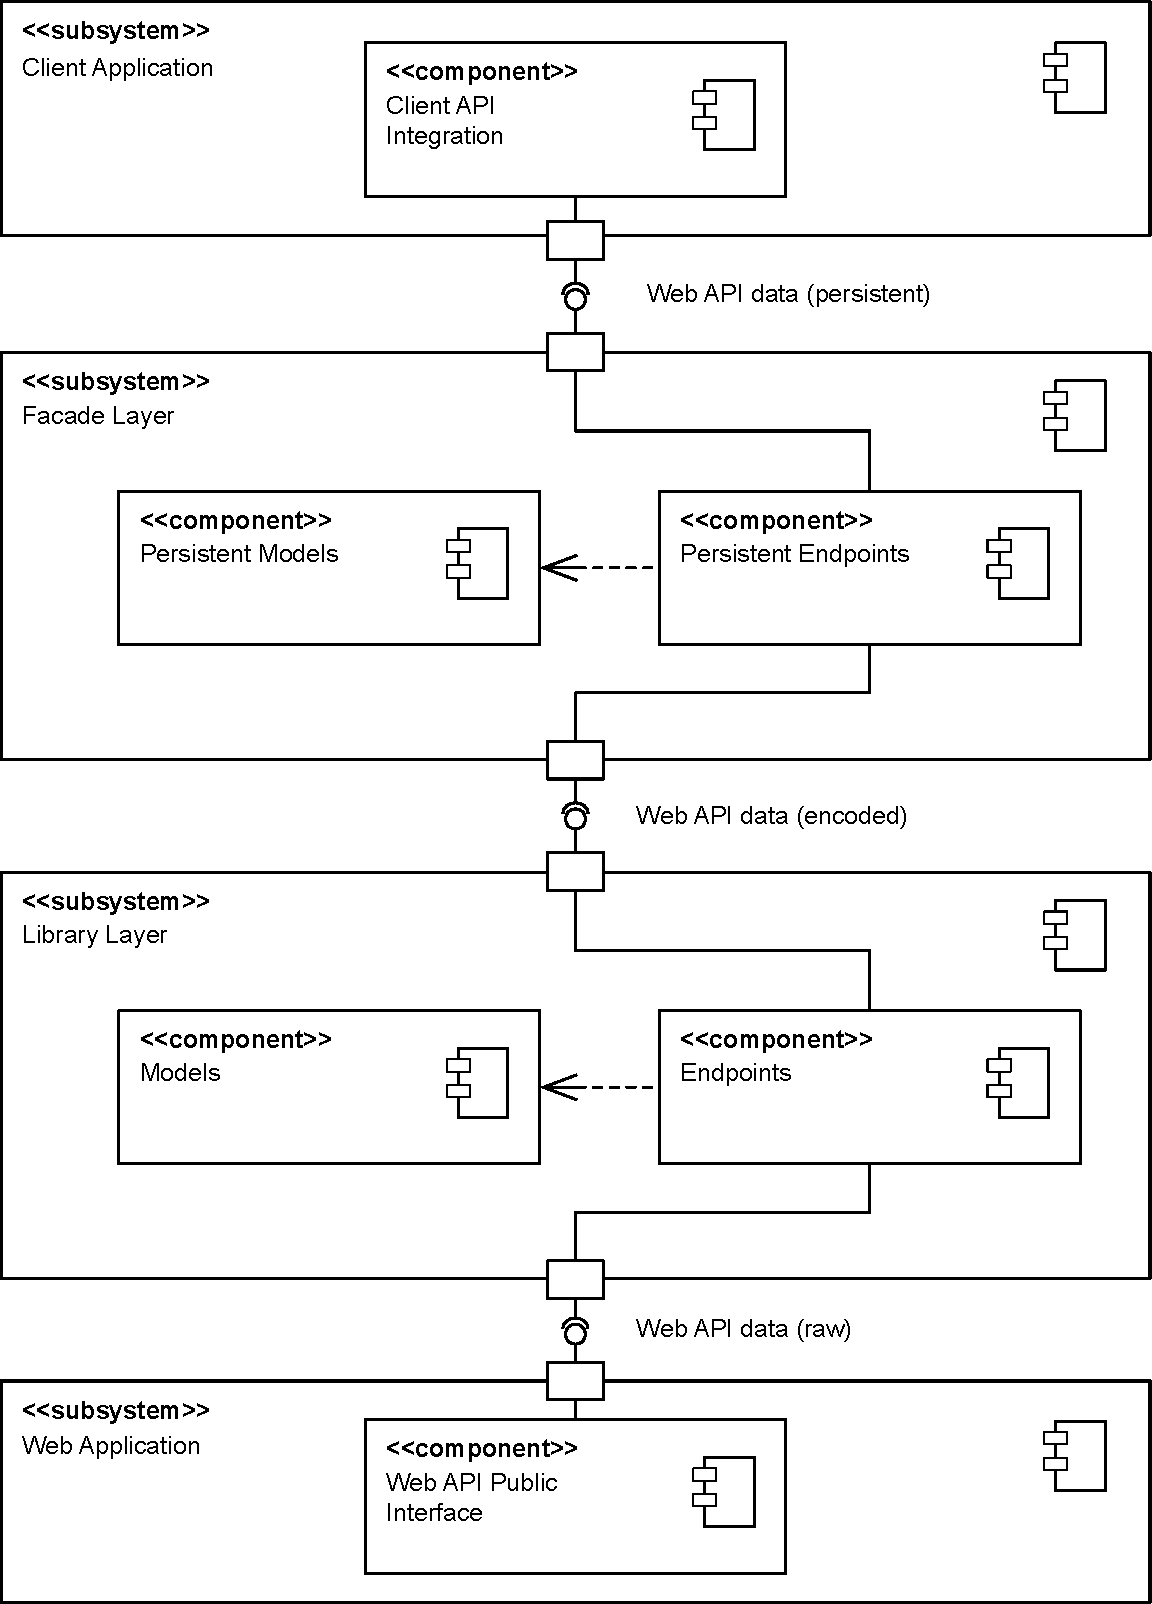
\includegraphics[width=130mm]{images/output_subsystem.pdf}
		\caption{Proposed architecture of change-proof Web API integration}
		\label{fig:outcome}
	}
\end{figure}

The output of our system is designed in a layered architectural style in order to incorporate changes made to the Web API without affecting the client application. Due to the fact that Web APIs are already integrated using a layered network architecture, introducing additional layers does not affect current development practices. The library subsystem is a local representation of the Web API and provides its services only to the facade subsystem. The facade subsystem uses them to issue HTTP requests to the Web API while maintaining a stable interface to the client application. When changes are introduced to the Web API, the library subsystem gets updated accordingly and the API contract between the library and facade subsystems is broken. For fixing the API contract, all changes stated in the migration guide modify the internal functionality of the facade subsystem without altering any publicly exposed interfaces. 

\subsection{Nonfunctional Requirements}
\label{subsec:NonfunctionalRequirements}
The following requirements were defined to ensure a high quality system. As described in \cite{bruegge_object-oriented_2010}, each requirement relates to one or more of the categories usability, reliability or supportability. According to the authors, supportability includes adaptability and maintainability.

\begin{itemize}[itemindent=-13pt, leftmargin=43pt, align=left]
    \item [NFR1\hphantom{1}] \customlabel{nfr:CodeStyle}{NFR1 (Code Style)} \textbf{Code Style:} All code generated by the system must follow a linting ruleset predefined in a configuration file to increase maintainability.
    \item [NFR2\hphantom{1}] \customlabel{nfr:ClientDocumentation}{NFR2} \textbf{Documentation of facade:} To increase usability for client application developers, the facade's public interface will be documented using code comments. These comments explain the usage of the Web API and are derived from its IDL document.
    \item [NFR3\hphantom{1}] \customlabel{nfr:SystemDocumentation}{NFR3} \textbf{Documentation of system:} To increase maintainability, the system will be documented using code comments. Documentation will be auto-gen\-erated and summarized in the \texttt{README.md} file.
    \item [NFR4\hphantom{1}] \customlabel{nfr:TestCoverage}{Test Coverage (NFR4)} \textbf{Test coverage:} To ensure the system's robustness, unit tests must be provided for all supported migration types. Additionally, unit test must be provided with respect to different migration strategies. Special attention needs to be paid to edge cases.
    \item [NFR5\hphantom{1}] \customlabel{nfr:Coloring}{NFR5}
    \textbf{Coloring of key messages:} Key output messages of the system will be highlighted using coloring schemes to increase usability.
    \item [NFR6\hphantom{1}] \customlabel{nfr:Help}{NFR6}
    \textbf{Help messages:} The system provides detailed instructions on how to use its command-line interface. The help will be available via \texttt{help} command. This ensures that users are able to easily learn how to operate the system.
    \item [NFR7\hphantom{1}] \customlabel{nfr:CodeVersion}{NFR7}
    \textbf{Code version:} The system is constrained to issuing language-specific library code in the language's current major version. This improves adaptability when client applications are using the latest version of a programming language.
    \item [NFR8\hphantom{1}] \customlabel{nfr:Dependencies}{NFR8}
    \textbf{Dependency Management:} Language-specific implementations are required to use a dependency manager to manage all third party libraries. Using a dependency manager increases maintainability significantly because dependency meta information provides a single source of truth.
        \item [NFR9\hphantom{1}] \customlabel{nfr:MigGuideFormat}{NFR9 (Migration Guide Format)}
    \textbf{Migration guide format:} The migration guide needs to be specified in a human-readable format which web developers are familiar with. Using a domain-specific language increases acceptance and usability especially for debugging and manual inspection. Additionally, utilizing a format that is already widely used in the software development industry has the advantage that IDEs provide convenient features such as syntax highlighting or auto-completion.
        \item [NFR10\hphantom{1}] \customlabel{nfr:UserInput}{NFR10}
    \textbf{Handling user input:} Missing or incorrect configuration parameters trigger a detailed error message so that the user can easily examine and correct the configuration.
\end{itemize}

\subsection{Constraints}
\label{subsec:Constraints}

For the system to work properly, some constraints have to be fulfilled. A constraint is a nonfunctional requirement that has been specified in advance by external factors and must be reconciled with other affected design decisions \cite{bass_software_2013}.

\begin{itemize}[itemindent=-13pt, leftmargin=43pt, align=left]
    \item [C1\hphantom{1}] \customlabel{nfr:Legal}{C1} \textbf{Legal requirements}: All dependencies must be available under MIT license regulations so that the system can also be published under the MIT license.
    \item [C2\hphantom{1}] \customlabel{nfr:Operations}{NFR2} \textbf{Operations requirements}: An IDL document describing the public interface of an API must be available in order to generate library code. Furthermore, both the API consumers and producers need to follow semantic versioning\footnote{see https://semver.org/} principles.
    \item [C3\hphantom{1}] \customlabel{nfr:Implementation}{NFR3} \textbf{Implementation requirements}: API consumers have to use GitHub as their version control system to use the system as a GitHub action in their CI/CD pipeline. Additionally, it is provided as a command-line program without a graphical user interface. This enables local execution or integration into other CI/CD tools.
\end{itemize}

\section{Use Cases}
\label{sec:UseCases}

After identifying requirements and constraints to enable an improved workflow for Web API consumers and providers, we derived use cases from their common interactions with our proposed system. Bruegge et. al define Use Cases as "general sequences of events that describe all the possible actions between an actor and the system for a given piece of functionality" \cite{bruegge_object-oriented_2010}.

For a better illustration we provide a use case diagram for both actors. Figure \ref{fig:useCaseConsumer} shows the typical use cases of our system from a Web API consumer's perspective.

\begin{figure}[h]
	\centering{
		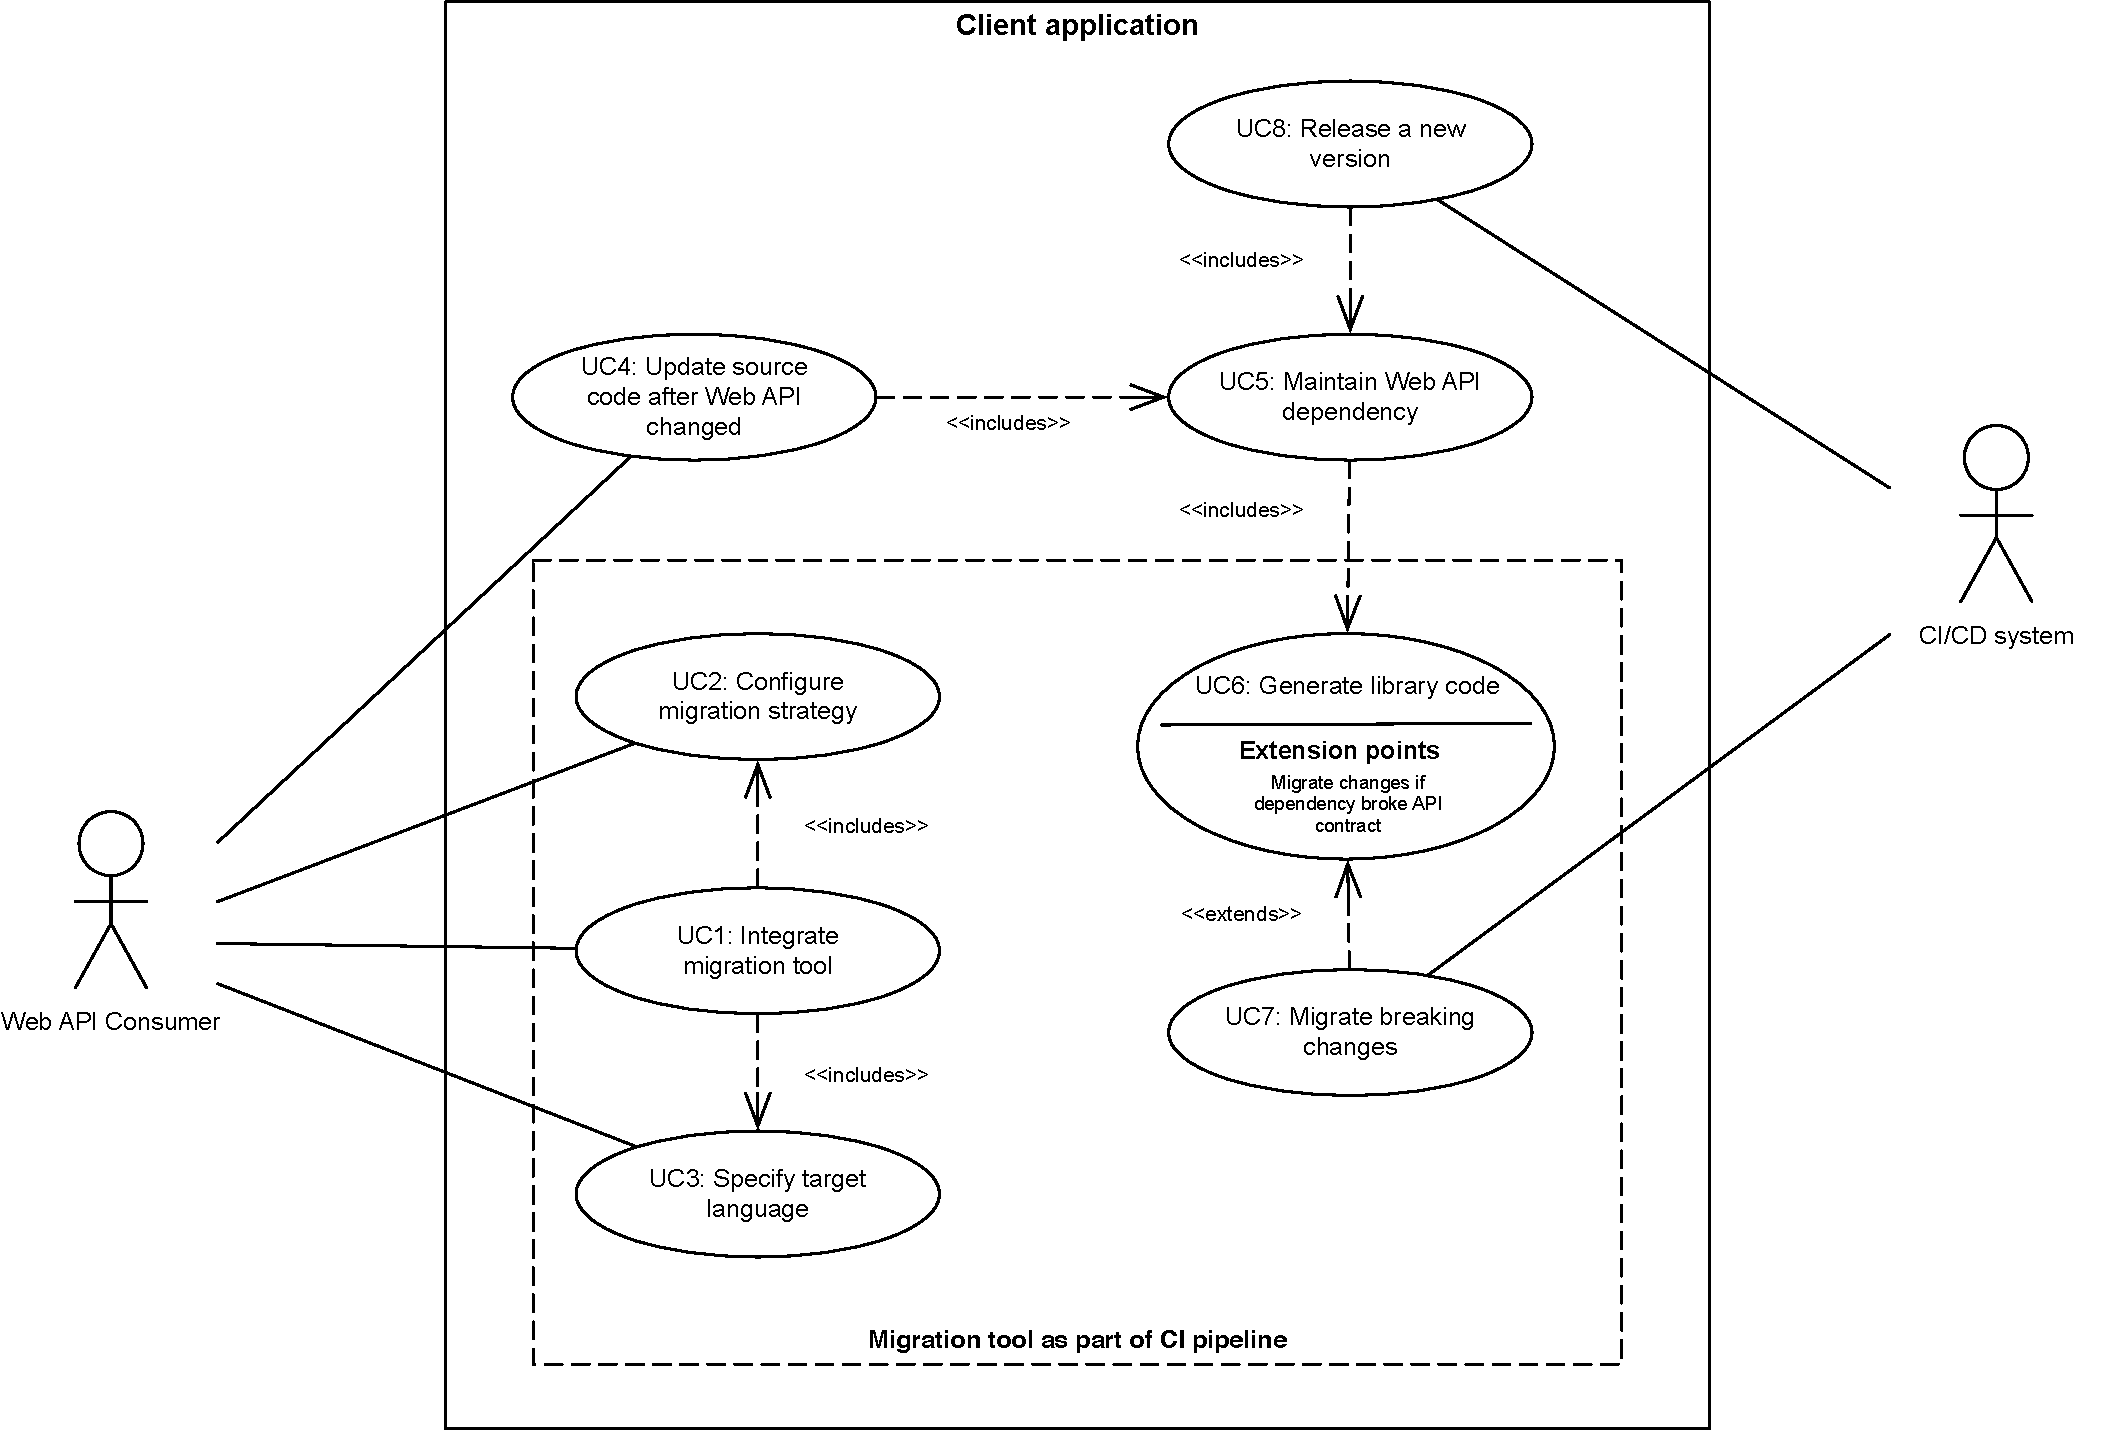
\includegraphics[width=155mm]{images/usecase_consumer.pdf}
		\caption{Use cases of Web API consumers}
		\label{fig:useCaseConsumer}
	}
\end{figure}

The migration tool is modeled as a subsystem of the client application due to its integration into the application's CI/CD pipeline. Integrating the tool requires Web API consumers to specify the target programming language for the generated library code. Furthermore, a migration strategy can be configured to meet the specific needs of the client project. Although both activities are part of the integration use case, they are modeled explicitly for client projects that do not use a CI/CD pipeline. 

Updating source code after a Web API dependency changed is the most important use case for Web API consumers. In addition to generating library code from a Web API's IDL document, our system migrates all changes as stated in its migration guide. This migration guide is created and published by Web API providers. The corresponding use case (\texttt{UC11}) is shown in figure \ref{fig:useCaseProvider}. 

The CI/CD system is modeled as a separate actor to illustrate the use cases that do not require manual interaction by client developers. Its primary task is to create a release of a new version of the client application without breaking changes that were introduced in the Web API. Therefore, it automatically migrates all of these changes by using our system.

For further explanation, the two most important use cases for Web API consumers are described in detail below.
\newpage
\subsubsection{Integrate Migration Tool}
\label{subsubsec:UseCase:IntegrateTool}

\vspace{-2mm}
\begin{center}
    \def\arraystretch{1.5}
    \begin{longtable}{ p{0.22\linewidth} p{0.72\linewidth} }
    \hline
        \textit{Source} & Web API consumer\\
    \hline
        \textit{Stimulus} & Client application needs to incorporate and persist a Web API. \\
    \hline
    	\textit{Environment} & \textbf{Preconditions:} The client application uses a CI / CD pipeline into which the migration tool can be integrated. The interface of the desired Web API is described using an IDL document.
    	
    	\textbf{Postcondition:} The resulting library must be added as a dependency to the client application.
    	\\
    \hline
    	\textit{Artefact} & Migration tool\\
    \hline
    \textit{Response} &
    \vspace{-5.1mm}
    \begin{enumerate}[itemindent=-9pt, leftmargin=14pt, itemsep=0pt, align=left]
    	\item The migration tool gets integrated as part of the CI/CD pipeline of the client application. Therefore, its configuration is either provided as a file via URI or via \ac{CLI} parameters. Optionally, a code formatting ruleset can be specified via its configuration file URI.
        \item The migration tool retrieves the IDL document from its URI.
        \item The migration tool parses the information from the IDL document and generates library code encapsulating lower level HTTP calls. This code is for internal use only and cannot be accessed publicly.
        \item The migration tool generates a public facade layer to persist the current view on the Web API by abstracting calls to the previously generated library code. 
        \item The migration tool generates related meta files to facilitate integrating the output via dependency management.
    \end{enumerate} \\ [-5mm]
    \hline
    \textit{Response Measure} &
    \vspace{-8.5mm}
    \begin{itemize}[itemindent=-9pt, leftmargin=14pt, itemsep=0pt, align=left]
       	\item Error: Execution fails if the IDL document is unavailable or incorrect.
       	\item Success: Output compiles and requests/responses to/from the Web API are processed without errors. 
        \vspace{-5mm}
    \end{itemize}\\
    \hline
    \end{longtable}
\end{center}
\newpage
\subsubsection{Update Source Code After Service Change}
\label{subsubsec:UseCase:FixClientApp}

\vspace{-2mm}
\begin{center}
    \def\arraystretch{1.5}
    \begin{longtable}{ p{0.22\linewidth} p{0.72\linewidth} }
    \hline
        \textit{Source} & Web API consumer\\
    \hline
        \textit{Stimulus} & The client application crashes after a modified Web API is published.\\
    \hline
    	\textit{Environment} & \textbf{Preconditions:} 
    	\begin{itemize}
    		\item The client application integrates a Web API via library code generated by our migration tool. 
    		\item Execution is either triggered manually or as part of a CI/CD pipeline of the client application. 
    		\item The latest release of a Web API introduced breaking changes either to its public interface or behavior. 
    		\item The Web API provider published a machine-readable migration guide along with an updated IDL document.
    	\end{itemize}
    	
    	\textbf{Postcondition:} Client application's dependency must be updated to use the latest version of the generated library code.
    	\\
    \hline
    	\textit{Artefact} & Migration tool\\
    \hline
    \textit{Response} &
    \vspace{-5.1mm}
    \begin{enumerate}[itemindent=-9pt, leftmargin=14pt, itemsep=0pt, align=left]
        \item The migration tool retrieves the updated IDL document and the migration guide from their URIs.
        \item The migration tool checks the changes specified in the migration guide for consistency and correctness. If this check fails, execution is aborted and an error is raised.
        \item The migration tool parses the information from the IDL document and generates library code encapsulating lower level HTTP calls. This code is for internal use only and cannot be accessed publicly.
        \item The migration tool uses the information from the migration guide to adapt the behavior of the previously generated facade layer without modifying the public interface of the facade.
        \item The migration tool generates related meta files to facilitate integrating the output via dependency management.
    \end{enumerate} \\ [-5mm]
    \hline
    \textit{Response Measure} &
    \vspace{-8.5mm}
    \begin{itemize}[itemindent=-9pt, leftmargin=14pt, itemsep=0pt, align=left]
    	\item Error: Execution fails if the IDL document is unavailable or incorrect.
       	\item Error: Execution fails if changes stated in the migration guide are contradicting or incompatible.
       	\item Success: Output compiles and requests/responses to/from the Web API are processed without errors. 
        \vspace{-5mm}
    \end{itemize}\\
    \hline
    \end{longtable}
\end{center}

Web API providers are the second group of actors that participate in our proposed workflow. Figure \ref{fig:useCaseProvider} shows the typical use cases of our system from their perspective.

\begin{figure}[h]
	\centering{
		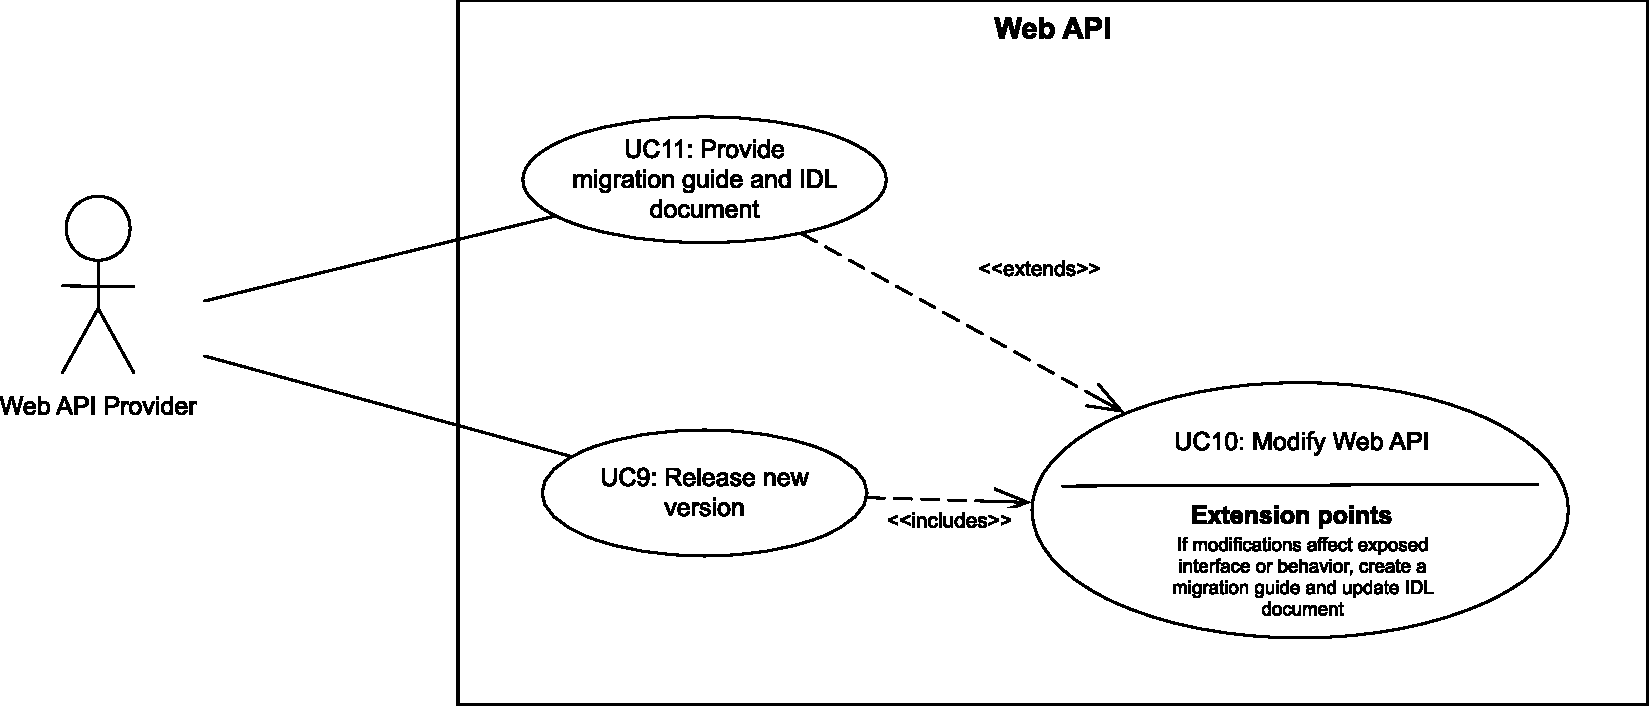
\includegraphics[width=150mm]{images/usecase_provider.pdf}
		\caption{Use cases of Web API providers}
		\label{fig:useCaseProvider}
	}
\end{figure}

Web API providers need to decide whether to introduce breaking changes to the publicly available interface or behavior. When breaking changes cannot be avoided, providers must create a machine-readable migration guide that specifies them. Furthermore, they need to provide an updated IDL document describing the current state of the Web API. Since our proposed workflow is only slightly different from their current workflow, a detailed description of a provider's use case focuses on providing a migration guide and an IDL document.

\subsubsection{Provide Migration Guide and IDL document}
\label{subsubsec:UseCase:MigGuideIDL}

\vspace{-2mm}
\begin{center}
    \def\arraystretch{1.5}
    \begin{longtable}{ p{0.22\linewidth} p{0.72\linewidth} }
    \hline
        \textit{Source} & Web API provider\\
    \hline
        \textit{Stimulus} & New functionality was added to the Web API or existing behavior was changed. Therefore, a new version of the Web API is released. \\
    \hline
    	\textit{Environment} & \textbf{Preconditions:} The provider introduced breaking changes to the exposed interface or behavior when modifying the Web API.
    	
    	\textbf{Postcondition:} The output needs to be published on a publicly accessible server and its URI has to be provided to Web API consumers.
    	\\
    \hline
    	\textit{Artefact} & Migration guide, IDL document\\
    \hline
    \textit{Response} &
    \vspace{-5.1mm}
    \begin{enumerate}[itemindent=-9pt, leftmargin=14pt, itemsep=0pt, align=left]
    	\item The IDL document must describe the publicly exposed interface and behavior. The Web API provider can either manually create this document or generate it using tools.
    	\item The migration guide must contain the type of IDL used to describe the Web API.
    	\item The migration guide must contain the type of Web API.
    	\item The migration guide must contain both the previous and the current version number according to the semantic versioning principles.
    	\item The migration guide can contain a short textual summary to provide an overview of the changes introduced in the current version.
    	\item The migration guide must contain a list of all breaking changes introduced in the current version. 
    \end{enumerate} \\ [-5mm]
    \hline
    \textit{Response Measure} &
    \vspace{-8.5mm}
    \begin{itemize}[itemindent=-9pt, leftmargin=14pt, itemsep=0pt, align=left]
       	\item Success: The migration guide can be retrieved and parsed by migration tool.
       	\item Success: The IDL document can be retrieved and parsed by migration tool.
        \vspace{-5mm}
    \end{itemize}\\
    \hline
    \end{longtable}
\end{center}

Currently, Web API providers have to manually create a migration guide. We propose that future research should explore automating this task to reduce the effort for providers. Existing tools for automatic generation of IDL documents can serve as a reference here.
\newpage
\section{Scenarios}
\label{sec:Scenarios}
According to Bruegge et. al, scenarios are instances of use cases describing a concrete set of actions \cite{bruegge_object-oriented_2010}. In the following section we present three example scenarios for possible uses of our system. They are intended to demonstrate how Web API providers and consumers can use our tool to simplify their respective workflows and meet the challenges of the independent evolution processes.

\subsubsection{Migrating an iOS application}
\label{subsubsec:Scenario:RESTScenario}

\textit{Simplified migration process in an iOS application that uses a REST API backend for storing and retrieving notes.}
\medskip
\\The iOS application "MyNotesApp" published by NoteMe Ltd. uses a REST API backend to store and retrieve the notes of its users. The backend utilizes the OpenAPI specification to describe its publicly exposed interface and behavior. Both systems are developed by individual teams that incorporate our migration tool into their workflow. Both code bases are located in separate repositories on GitHub\footnote{https://www.github.com/}. After Alice, a developer from the backend team, published a new version of the REST API, she provides two URIs located on the same web server pointing to the updated OpenAPI specification and a migration guide. Since new business demands required her to modify the application's data models, breaking changes were introduced that she specified in the migration guide. Bob, a member of the frontend developer team is aware of these breaking changes, but he cannot apply all changes manually because the frontend team faces staffing shortage. However, our migration tool is part of the CI pipeline as a GitHub action, which automatically migrates all changes and generates updated library code that is submitted via git pull request to its own repository on GitHub. Since the iOS application uses the Swift Package Manager to maintain its dependencies, the updated library code is automatically incorporated after the frontend team accepted the pull request. A new release is created by the CD system and Claire, the tech leader of "MyNotesApp" publishes the app to the Apple AppStore.
\subsubsection{Migrating a web application using a third party service}
\label{subsubsec:Scenario:gRPCScenario}

\textit{Simplified migration process in a web application that uses a public gRPC-based API provided by Google to create 3D animated GIFs.}
\medskip
\\ The social media platform "Yearbook" is a web application written in TypeScript, that enables users to share the most important milestones of their year. It differs from other platforms in that the number of posts per user is limited to 12 posts per year. SocialViz Inc., the company behind Yearbook, identified that its customers want to use animated GIFs to celebrate their birthdays with their friends and families with an eye-catching post. Creating a GIF is an inconvenient process for their users. Fortunately, Google LLC provides "gifinator", a public service that allows client applications to create animated 3D GIFs by sending gRPC-based messages with parameters specifying the style of these animations. Lucas, a developer on the Yearbook frontend team, is responsible for integrating this interface. Since Google released the API in a beta version, it is subject to frequent, unannounced changes, namely renaming of public operations. Lucas spends a large share of his working hours adjusting the interface to adapt to these changes while his other tasks remain unfinished. To meet these challenges, he integrates our tool into the CI pipeline of Yearbook. Thereby, all changes are automatically incorporated and abstracted, generating a stable interface that client code can rely on. To make this possible, Google offers a machine-readable migration guide and an updated \texttt{.proto} file, that are fetched by our system. Since the generated output is built into the Yearbook as a JavaScript library, updating this dependency can easily be done by Lucas, who publishes it on a web server.
\subsubsection{Automating migration documentation for Web API providers}
\label{subsubsec:Scenario:graphQLScenario}

\textit{Simplified evolution process for the provider of a GraphQL-based Web API by generating a machine-readable migration guide that can be used by the consumer's tools}
\medskip
\\ "Unsensored" is an application of the startup Ingenuitees. It collects and analyzes sensor information from industrial machines to predict the need for maintenance activities. After they built a solid customer base and sufficient industry knowledge, they want to expand their services to new potential customers. Therefore, they decided to create a monetized Web API that allows to query analytical information using the GraphQL query language and incorporate the responses in client applications. As they work closely with their customers, Amanda, Ingenuitees 'senior developer, presents their plan to Drew, a developer responsible for integrating third-party services at OnTrack Ltd., one of Ingenuitees' key customers. Although Drew likes this idea, he points out that OnTrack Ltd. has strict requirements for the stability of API contracts. These requirements are at odds with Ingenuitee's entrepreneurial spirit and agile development processes. Therefore, Amanda wants to ensure that new features can be added frequently while deprecated features can be changed without breaking client applications. Drew advises her that he has included our proposed system in their application's CI pipeline to automatically migrate other third-party Web APIs. For this to work, Amanda would have to state every change in a machine-readable migration guide and provide it along with the new version and IDL document. They agree to develop a proof of concept, whereupon Amanda begins to gather information regarding the creation of a migration guide. She finds that by comparing the differences in the schema definitions of two versions of their API, she can develop an algorithm to generate a machine-readable migration guide. She integrates this algorithm as a Github action into the CI pipeline of the Web API and publishes the result along with the updated schema definition on a staging web server. Drew uses our system to integrate the Web API of "Unsensored" in their test environment. After verifying that the migrations are done correctly, Amanda publishes the Web API for production.